\documentclass{beamer}

\usepackage{comment}
\usepackage{color}
\usepackage{listings}
\usepackage{verbatim}
\usepackage{multicol}
\usepackage{booktabs}
\definecolor{green}{RGB}{0,128,0}

\newcommand\gehcomment[1]{{{\color{orange} #1}}}
\newcommand\add[1]{{{\color{blue} #1}}}
\newcommand\remove[1]{\sout{{\color{red} #1}}}
\newcommand\codecomment[1]{{{\color{green} #1}}}
\newcommand\redcomment[1]{{{\color{red} #1}}}
\newcommand\bluecomment[1]{{{\color{blue} #1}}}
\newcommand\greencomment[1]{{{\color{green} #1}}}
\newcommand\magentacomment[1]{{{\color{magenta} #1}}}

\begin{comment}
\tiny
\scriptsize
\footnotesize
\small
\normalsize
\large
\Large
\LARGE
\huge
\Huge
\end{comment}

\begin{document}
\title{Multiphase - Gas Injection}
\author{Emily Stein}
\date{\today}

%\frame{\titlepage}

%-----------------------------------------------------------------------------
\section{Description of GDSA}

\subsection{GDSA Conceptual Model}

\begin{frame}\frametitle{Description of Geologic Disposal Scenario}
The ``Geologic Disposal Scenario'' demonstrates how to use the process models developed specifically for performance assessment simulations of deep geologic nuclear waste repositories, including WASTE\_FORM, UFD\_DECAY, and UFD\_BIOSPHERE.
\begin{itemize}
  \item Problem domain: $3000 \times 5 \times 1005$ m (x $\times$ y $\times$ z)
  \item Grid resolution: Varies in an unstructured grid
  \item Flow mode: TH (thermal/hydro)
  \item Heat Source: Rate scaled by cell volume
  \item Radionuclide Sources: Defined with WASTE\_FORM
  \item Radionuclide Behavior: Controlled by UFD\_DECAY
  \item Dose: Calculated with UFD\_BIOSPHERE
  \item Total simulation time: 500,000 y
\end{itemize}

\end{frame}

%-----------------------------------------------------------------------------
\frame{\frametitle{Geologic Disposal Schematic}
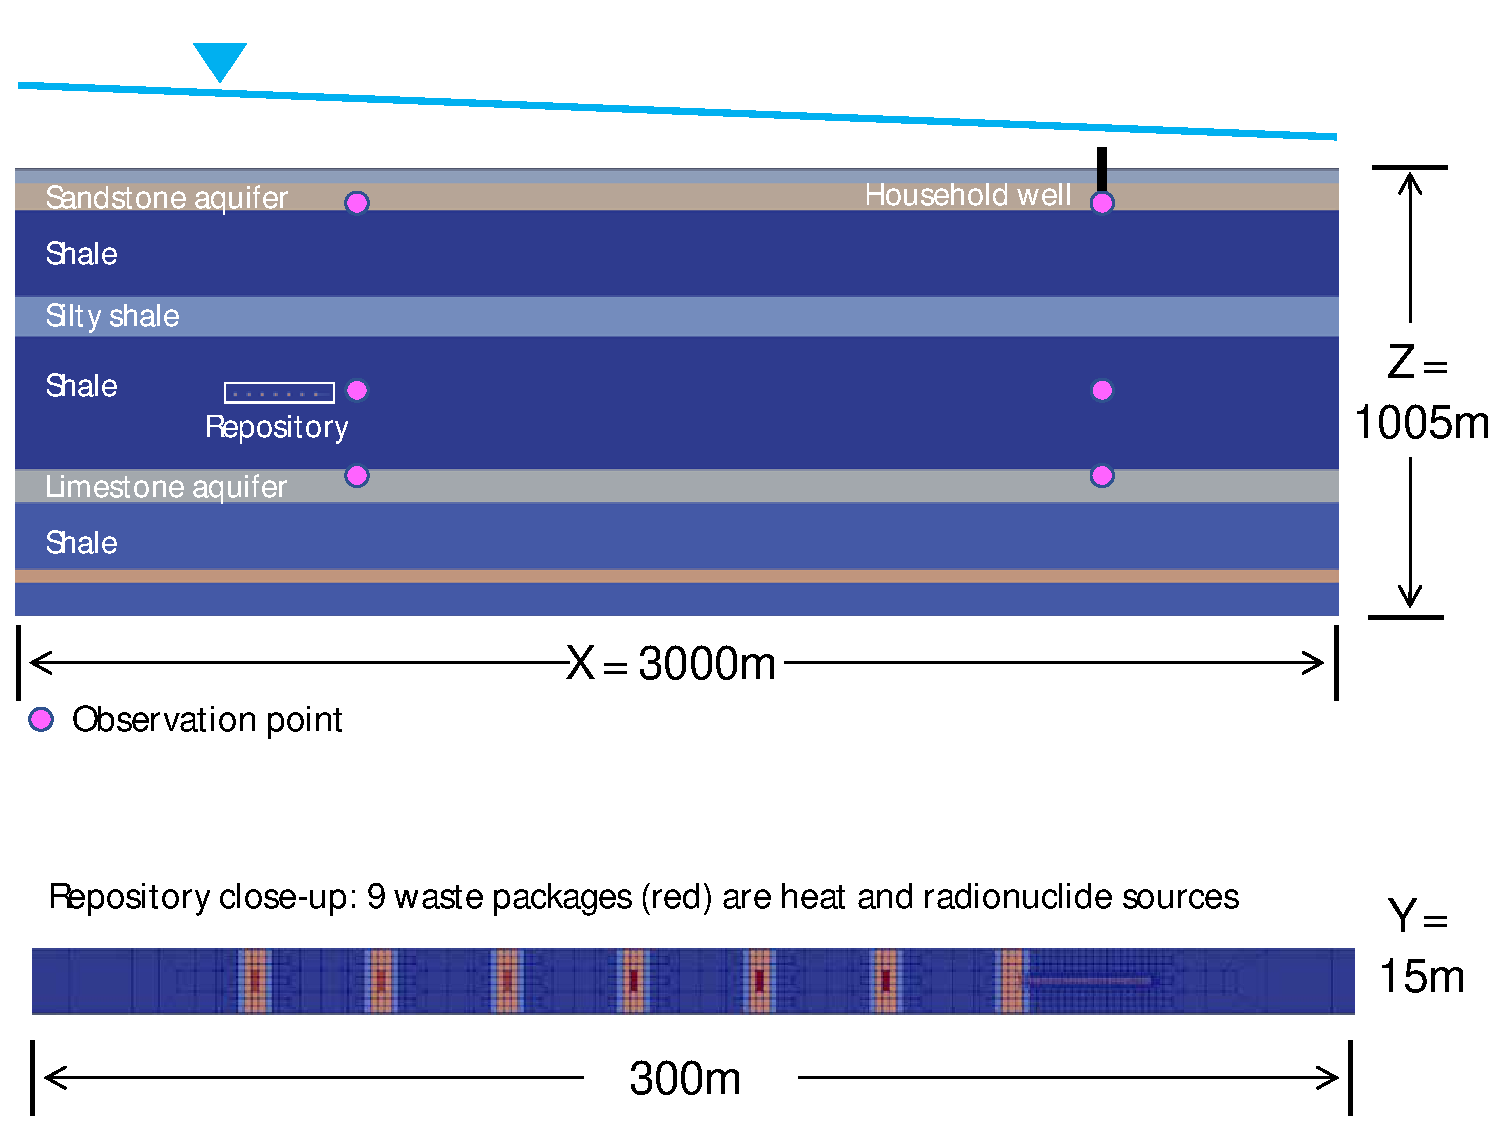
\includegraphics[width=\linewidth]{./gdsa_schematic}
}

%-----------------------------------------------------------------------------
\frame{\frametitle{Geologic Disposal Initial Conditions}
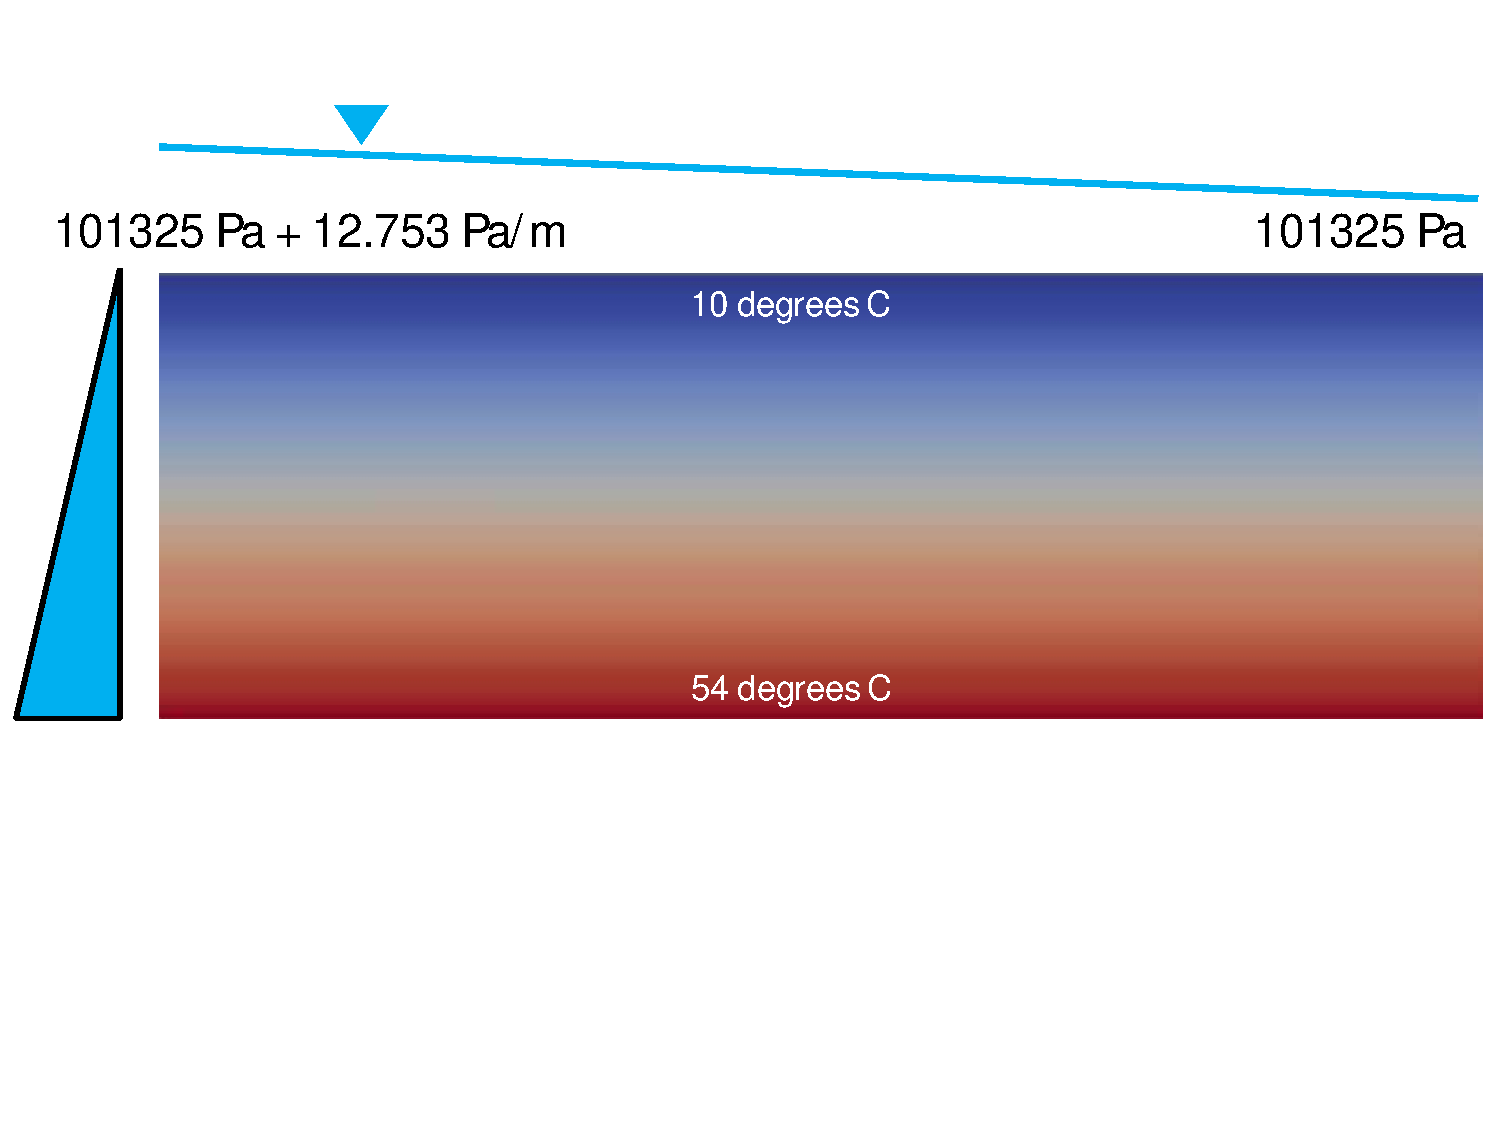
\includegraphics[width=\linewidth]{./gdsa_ic}
}

%-----------------------------------------------------------------------------
\section{Partial Description of Input Deck}

%-----------------------------------------------------------------------------
\subsection{SIMULATION}

\begin{frame}[fragile]\frametitle{SIMULATION}

\begin{itemize}
  \item Specify Process Models
\end{itemize}

\begin{semiverbatim}\small
SIMULATION
  SIMULATION_TYPE SUBSURFACE
  PROCESS_MODELS
    SUBSURFACE_FLOW flow
      MODE TH \bluecomment{! thermal/hydro}
      OPTIONS
        MAX_PRESSURE_CHANGE 1.d8 \bluecomment{! Pa}
      /   
    /   
    SUBSURFACE_TRANSPORT transport
      GLOBAL_IMPLICIT
    /
    UFD_DECAY ufd_decay \bluecomment{! in aqueous, solid, and sorbed phases}
    /
    WASTE_FORM wf_general \bluecomment{! waste package and waste form degradation}
    /
    UFD_BIOSPHERE bio \bluecomment{! dose calculation at a drinking well}
    /
  /
END
\end{semiverbatim}

\end{frame}

%-----------------------------------------------------------------------------
\subsection{DATASET}

\begin{frame}[fragile]\frametitle{DATASET}

\begin{itemize}
  \item Used for initial and boundary conditions
\end{itemize}

\begin{semiverbatim}
DATASET 1d_temperature
  FILENAME ./initcond/reggrad0013.h5
  HDF5_DATASET_NAME hydrostatic_boundary_T
/
DATASET 1d_pressure
  FILENAME ./initcond/reggrad0013.h5
  HDF5_DATASET_NAME hydrostatic_boundary_P
/
\end{semiverbatim}

\end{frame}

%-----------------------------------------------------------------------------
\subsection{CHEMISTRY}

\begin{frame}[fragile]\frametitle{CHEMISTRY}

\begin{itemize}
  \item Aqueous and solid phase for each radionuclide
\end{itemize}

\begin{semiverbatim}
CHEMISTRY
  PRIMARY_SPECIES
    Am241
    Am243
    ...
    I129
    Cs135
  /
  MINERALS
    Am241(s)
    Am243(s)
    ...
    I129(s)
    Cs135(s)
  /
\end{semiverbatim}

\end{frame}

%-----------------------------------------------------------------------------
\begin{frame}[fragile]\frametitle{CHEMISTRY}

\begin{itemize}
  \item Rate constants = 0
\end{itemize}

\begin{semiverbatim}
  MINERAL_KINETICS
    Am241(s)
      RATE_CONSTANT 0.0d0
    /
    \bluecomment{...}
    Cs135(s)
      RATE_CONSTANT 0.0d0
    /
  /
  TRUNCATE_CONCENTRATION 1.d-21
  DATABASE ./ufd-decay.dat
  OUTPUT
    TOTAL
    TOTAL_SORBED
    ALL
  /
END
\end{semiverbatim}

\end{frame}

%-----------------------------------------------------------------------------
\subsection{GRID}

\begin{frame}[fragile]\frametitle{GRID}

\begin{itemize}
  \item Implicit unstructured grid 
\end{itemize}

\begin{semiverbatim}
GRID
  TYPE UNSTRUCTURED ./gdsa_usg.h5
END
\end{semiverbatim}

\end{frame}

%-----------------------------------------------------------------------------
\subsection{TIME}

\begin{frame}[fragile]\frametitle{TIME}
\begin{itemize}
  \item Final simulation time = 500,000 y
\end{itemize}

\begin{semiverbatim}

TIME
  FINAL_TIME 5.d5 y
  INITIAL_TIMESTEP_SIZE 1.d-6 y
  MAXIMUM_TIMESTEP_SIZE 1. y at 1. y
  MAXIMUM_TIMESTEP_SIZE 5. y at 10. y
  MAXIMUM_TIMESTEP_SIZE 50. y at 100. y
  MAXIMUM_TIMESTEP_SIZE 500. y at 1000. y
  MAXIMUM_TIMESTEP_SIZE 5000. y at 10000. y
END
\end{semiverbatim}

\end{frame}

%-----------------------------------------------------------------------------
\subsection{OUTPUT}

\begin{frame}[fragile]\frametitle{OUTPUT}
\begin{itemize}
  \item Print a snapshot of entire solution periodically
  \item Print the solution at observation points every time step
  \item Print mass balance file every time step
  \item Choose output variables
\end{itemize}

\end{frame}

\begin{frame}[fragile]\frametitle{OUTPUT}

\begin{semiverbatim}\small
OUTPUT
  SNAPSHOT_FILE
    FORMAT HDF5
    PRINT_COLUMN_IDS \bluecomment{! useful for plotting}
    PERIODIC TIME 1. y between 0. y and 10. y  \bluecomment{! every year}
    PERIODIC TIME 10. y between 0. y and 100. y  \bluecomment{! then every 10 y}
    \bluecomment{! see input deck for more}
  /
  OBSERVATION_FILE
    PERIODIC TIMESTEP 1 \bluecomment{! print every time step}
  /
  MASS_BALANCE_FILE
    PERIODIC TIMESTEP 1 \bluecomment{! print every time step}
  /
  VELOCITY_AT_CENTER \bluecomment{! of cell}
  VARIABLES
    TEMPERATURE
    LIQUID_PRESSURE \bluecomment{! see input deck for more}
  /
END
\end{semiverbatim}

\end{frame}

%-----------------------------------------------------------------------------
\subsection{EXTERNAL\_FILE}

\begin{frame}[fragile]\frametitle{EXTERNAL\_FILE}
\begin{itemize}
  \item Use the contents of another file in the input deck
\end{itemize}

\begin{semiverbatim}
EXTERNAL_FILE ./obs_points.txt \bluecomment{! OBSERVATION blocks}
\end{semiverbatim}

\begin{itemize}
  \item Elsewhere this input deck contains multiple EXTERNAL\_FILEs
\end{itemize}

\begin{semiverbatim}
EXTERNAL_FILE ./regions.txt \bluecomment{! REGION blocks}
EXTERNAL_FILE ./obs_regions.txt \bluecomment{! REGION blocks used for OBSERVATION} 
EXTERNAL_FILE ./source_sink.txt \bluecomment{! SOURCE_SINK blocks for heat}
EXTERNAL_FILE ./strata.txt \bluecomment{! STRATA blocks}
EXTERNAL_FILE ./wfg.txt \bluecomment{! WASTE_FORM blocks}
\end{semiverbatim}

\end{frame}

%-----------------------------------------------------------------------------
\subsection{FLUID\_PROPERTY}

\begin{frame}[fragile]\frametitle{FLUID\_PROPERTY}
\begin{itemize}
  \item Free water diffusion coefficient
\end{itemize}

\begin{semiverbatim}
FLUID_PROPERTY
  PHASE LIQUID
  DIFFUSION_COEFFICIENT 1.d-9
END
\end{semiverbatim}

\end{frame}

%-----------------------------------------------------------------------------
\subsection{MATERIAL\_PROPERTY}

\begin{frame}[fragile]\frametitle{MATERIAL\_PROPERTY}
\begin{itemize}
  \item Input deck contains 12 MATERIAL\_PROPERTY blocks
  \item One example shown below
\end{itemize}

\begin{semiverbatim}\small
MATERIAL_PROPERTY shale
  ID 1
  SATURATION_FUNCTION default
  POROSITY 0.20
  TORTUOSITY_FUNCTION_OF_POROSITY 1.4
  SOIL_COMPRESSIBILITY 1.6d-8 #1/Pa
  SOIL_COMPRESSIBILITY_FUNCTION DEFAULT
  SOIL_REFERENCE_PRESSURE 101325.d0
  ROCK_DENSITY 2700.
  THERMAL_CONDUCTIVITY_DRY 1.2d0 ! not used
  THERMAL_CONDUCTIVITY_WET 1.2d0
  HEAT_CAPACITY 830.
  PERMEABILITY
    PERM_ISO 1.d-19
  /
/
\end{semiverbatim}
\end{frame}

%-----------------------------------------------------------------------------
\subsection{CHARACTERISTIC\_CURVES}

\begin{frame}[fragile,containsverbatim]\frametitle{SATURATION\_FUNCTION}
\begin{itemize}
  \item TH mode syntax
\end{itemize}
\begin{semiverbatim}\small
SATURATION_FUNCTION default
  SATURATION_FUNCTION_TYPE VAN_GENUCHTEN
  RESIDUAL_SATURATION 0.1d0
  LAMBDA 0.5
  ALPHA 1.d-4
END
\end{semiverbatim}
\end{frame}

%-----------------------------------------------------------------------------
\subsection{FLOW\_CONDITION}

\begin{frame}[fragile]\frametitle{FLOW\_CONDITION}
\begin{itemize}
  \item{Using datasets}
\end{itemize}

\begin{semiverbatim}
FLOW_CONDITION initial \bluecomment{! also for boundary conditions}
  TYPE
    PRESSURE DIRICHLET
    TEMPERATURE DIRICHLET
  /
  PRESSURE DATASET 1d_pressure
  TEMPERATURE DATASET 1d_temperature
END

\end{semiverbatim}
\end{frame}

\begin{frame}[fragile]\frametitle{FLOW\_CONDITION}
\begin{itemize}
  \item{3 heat sources from files}
  \item{one shown for example}
\end{itemize}

\begin{semiverbatim}
FLOW_CONDITION hlw
  TYPE
    RATE MASS_RATE
    ENERGY_RATE SCALED_ENERGY_RATE VOLUME \bluecomment{! distribute by volume}
  /
  \bluecomment{!SYNC_TIMESTEP_WITH_UPDATE}
  INTERPOLATION LINEAR \bluecomment{interpolate between times in the file}
  RATE 0.d0 \bluecomment{! liquid flux rate}
  ENERGY_RATE FILE ./hlw_heat.txt \bluecomment{! contains list of time, watts}
END

\end{semiverbatim}
\end{frame}

\begin{frame}[fragile]\frametitle{FLOW\_CONDITION}
\begin{itemize}
  \item{hlw\_heat.xt}
\end{itemize}

\begin{semiverbatim}\small
TIME_UNITS y
DATA_UNITS W
# time energy (W/waste package)
0.00E+00        1.755E+02
1.00E-01        1.751E+02
2.00E-01        1.747E+02
3.00E-01        1.743E+02
4.00E-01        1.739E+02
5.00E-01        1.735E+02
6.00E-01        1.732E+02
7.00E-01        1.728E+02
8.00E-01        1.724E+02
9.00E-01        1.720E+02
1.00E+00        1.716E+02
\bluecomment{...}
2.00E+05        6.631E-02
5.00E+05        6.488E-02
/
\end{semiverbatim}
\end{frame}

%-----------------------------------------------------------------------------
\subsection{END\_SUBSURFACE}
\begin{frame}[fragile]\frametitle{END\_SUBSURFACE}

\begin{itemize}
  \item Close the SUBSURFACE block
\end{itemize}

\begin{semiverbatim}
END_SUBSURFACE \bluecomment{! WASTE_FORM, UFD_DECAY, UFD_BIOSPHERE follow}
\end{semiverbatim}
\end{frame}

%-----------------------------------------------------------------------------
\subsection{WASTE\_FORM}
\begin{frame}[fragile]\frametitle{WASTE\_FORM GENERAL}

\begin{itemize}
  \item WASTE\_FORM block for each waste package
  \item MECHANISM block for each kind of waste
\end{itemize}

\begin{semiverbatim}\small
WASTE_FORM_GENERAL
  \bluecomment{! individual waste package regions are in:}
  EXTERNAL_FILE ./wfg.txt
  PRINT_MASS_BALANCE \bluecomment{! optional}
\end{semiverbatim}

\begin{itemize}\small
  \item Example WASTE\_FORM block in wfg.txt
\end{itemize}

\begin{semiverbatim}
  WASTE_FORM
     REGION hlw0 \bluecomment{! a waste package}
     EXPOSURE_FACTOR 5.416057 \bluecomment{! adjust surface area}
     VOLUME 9.500000 \bluecomment{! m^3}
     MECHANISM_NAME hlw \bluecomment{! reference to inventory}
  /
\end{semiverbatim}
\end{frame}
%-----------------------------------------------------------------------------
\subsection{UFD\_DECAY}
\begin{frame}[fragile]\frametitle{UFD\_DECAY}

\begin{itemize}
  \item Solubility limits and sorption coefficients for each element
  \item Decay rates and daughters for each isotope
\end{itemize}

\begin{semiverbatim}\small
UFD_DECAY
  ELEMENT I
    SOLUBILITY 1.d4 \bluecomment{! mol/L}
    KD \bluecomment{! kg water / m^3 bulk}
      metallic 0.d0
      hlw 0.d0
      oxide 0.d0
      buffer 0.d0
      shale 0.d0
      drz 0.d0
      siltstone 0.d0
      sandstone 0.d0
      limestone 0.d0
      lower_shale 0.d0
      overburden 0.d0
      lower_sandstone 0.d0
    /
  /
  ISOTOPE I129
    ELEMENT I
    DECAY_RATE 1.29d-15 \bluecomment{! 1/s}
    \bluecomment{!DAUGHTER Xe129 1.d0}
  /
  \bluecomment{...}
END \bluecomment{! UFD_DECAY}
\end{semiverbatim}
\end{frame}

%-----------------------------------------------------------------------------
\subsection{UFD\_BIOSPHERE}
\begin{frame}[fragile]\frametitle{UFD\_BIOSPHERE}

\begin{itemize}
  \item Information about well and individual consumption
  \item Sorption coefficient, decay rate, and dose coefficient
\end{itemize}

\begin{semiverbatim}\small
UFD_BIOSPHERE
  ERB_1B B_model1 \bluecomment{! use this model without a sink}
    REGION fake_well \bluecomment{! does not pump}
    DILUTION_FACTOR 1.0 \bluecomment{! use dilution factor instead}
    INDIVIDUAL_CONSUMPTION_RATE 2.d0 L/day
    \bluecomment{! INCLUDE_UNSUPPORTED_RADS}
  /

  SUPPORTED_RADIONUCLIDES
    RADIONUCLIDE I129
      ELEMENT_KD 0.d0  # L-water/kg-solid average in vicinity of well screen
      DECAY_RATE 1.40d-15 1/sec
      INGESTION_DOSE_COEF 1.1d-7 Sv/Bq
    /
    \bluecomment{...}
  /
  OUTPUT_START_TIME 1.d4 y
END \bluecomment{! UFD_BIOSPHERE}
\end{semiverbatim}
\end{frame}

%-----------------------------------------------------------------------------
\subsection{Command Line}
\begin{frame}[fragile]\frametitle{Command Line}

\begin{itemize}
  \item Run the simulation
\end{itemize}
\begin{semiverbatim}
\$ pflotran -input_prefix gdsa
\end{semiverbatim}

\end{frame}

\begin{frame}[fragile]\frametitle{Command Line}

\begin{itemize}
  \item Plot the results
\end{itemize}

\begin{semiverbatim}
\$ python gdsa.py
\end{semiverbatim}

\end{frame}

%-----------------------------------------------------------------------------
\end{document}
